   %\documentclass[wcp,gray]{jmlr} % test grayscale version
\documentclass[wcp]{jmlr}


%% Personnal package
\usepackage{enumerate}
\usepackage{bbold}
\usepackage{wrapfig}


 % The following packages will be automatically loaded:
 % amsmath, amssymb, natbib, graphicx, url, algorithm2e

 %\usepackage{rotating}% for sideways figures and tables
% \usepackage{longtable}% for long tables

 % The booktabs package is used by this sample document
 % (it provides \toprule, \midrule and \bottomrule).
 % Remove the next line if you don't require it.
\usepackage{booktabs}
 % The siunitx package is used by this sample document
 % to align numbers in a column by their decimal point.
 % Remove the next line if you don't require it.
\usepackage[load-configurations=version-1]{siunitx} % newer version
 %\usepackage{siunitx}
\usepackage[utf8]{inputenc}

 % The following command is just for this sample document:
\newcommand{\cs}[1]{\texttt{\char`\\#1}}

% % Define an unnumbered theorem just for this sample document:
%\theorembodyfont{\upshape}
%\theoremheaderfont{\scshape}
%\theorempostheader{:}
%\theoremsep{\newline}
%\newtheorem*{note}{Note}

 % change the arguments, as appropriate, in the following:
\jmlrvolume{1}
\jmlryear{2014}
\jmlrworkshop{\textcolor{red}{Neural Connectomics Workshop}}

% \title[Connectomics challenge]{Inferring neural networks from fluorescent
%                                calcium imaging using partial correlation and
%                                sample weighting \textcolor{red}{plus court} : Simple and robust inference of connectomes using partial correlation coefficients
% ?}

% \title[Inference of connectomes using partial correlation coefficients]{Simple and robust inference of connectomes using partial correlation coefficients}

\title{\textcolor{red}{Simple} connectome inference using partial correlation from imaging calcium signal}


% %%
% Discovery/Infering/Retrieving/... connectomes
% Robust
% Using partial correlation
% [from calcium imaging]


 % Use \Name{Author Name} to specify the name.
 % If the surname contains spaces, enclose the surname
 % in braces, e.g. \Name{John {Smith Jones}} similarly
 % if the name has a "von" part, e.g \Name{Jane {de Winter}}.
 % If the first letter in the forenames is a diacritic
 % enclose the diacritic in braces, e.g. \Name{{\'E}louise Smith}

 % Two authors with the same address
%  \author{\Name{Author Name1\nametag{\thanks{with a note}}} \Email{abc@sample.com}\and
%   \Name{Author Name2} \Email{xyz@sample.com}\\
%   \addr Address}

 % Three or more authors with the same address:
 % \author{ Antonio Sutera %\and
 %         % \Name{Arnaud Joly} \and
 %         % \Name{Vincent Fran\c{c}ois-Lavet} \and
 %         % \Name{Aaron Qiu} \and
 %         % \Name{Gilles Louppe} \and
 %         % \Name{Damien Ernst} \and
 %         % \name{Pierre Geurts}}
 %         }
\author{Antonio Sutera,
        Arnaud Joly,
        Vincent François-Lavet,
        Aaron Qiu, \\
        Gilles Louppe,
        Damien Ernst,
        Pierre Geurts}

 % Authors with different addresses:
 % \author{\Name{Author Name1} \Email{abc@sample.com}\\
 % \addr Address 1
 % \AND
 % \Name{Author Name2} \Email{xyz@sample.com}\\
 % \addr Address 2
 %}

\editor{Editor's name}
 % \editors{List of editors' names}

\begin{document}

\maketitle


\begin{abstract}
Understanding how the brain works is a key
to treat brain disorders such as Parkinson's disease,
epilepsy. Retrieving connectomes, the neurons wiring map, will shed a new
light on the anatomical and functional connectivity of the brain. In the
context of the Connectomics challenge, we propose a simple  algorithm made of
four stages, using preprocessing and partial correlation to achieve a network
inference of high quality. We put in perspective our method
with other inference methods such as GTE (\cite{stetter2012model}) and Genie3
(\cite{huynhthu2010inferring}).

% Discussion on the metrics?
%\textcolor{red}{Discussion on the order of the partial correlation}

\end{abstract}

\begin{keywords}
Network inference - Partial correlation - Precision matrix - GENIE3
\end{keywords}


\section{Introduction}\label{sec:intro}

% BG : brain, complex organ
The human brain is a complex biological organ, formed by 100
billions of neurons with 7000 synaptic connections on average.
Cutting edge optical devices have been developed to track in real-time
the neuronal activity of thousands of neurons through a fluorescent
calcium indicator  [todo cite]. Automatic and analytical methods are required to infer
the connectomes from those time series.

% Introduce notation + goal in mathematical score
% TODO check convention for y_{ij}
The connectomes, the neural network, is represented by a (un)directed graph $G = (V, E)$ comprising
a set of nodes $V$ and a set of edges $E \subseteq \left\{(i, j) \in V \times
V\right\}$, (un)ordered pair from $V$.
Each node $i \in V$ represents a neuron, and each edge $(i, j) \in E$
represents a direct link from a neuron $i$ to a neuron $j$.
The network inference task is set as follows :
\textit{Given the observations $(x_t \in \mathcal{R}^{|V|})_{t=1}^T $
along $T$ periods of time of the $|V|$ neurons, the goal is to infer the
adjacency matrix $A : a_{i,j} = \mathbb{1}((i, j) \in E)$ of the neural network
of graph $G$, where $\mathbb{1}$ is the indicator function.}

% Solution
In this paper, we describe a simple and a theoretically grounded approach
based on partial correlation\footnote{Source code is available at
\url{https://github.com/asutera/kaggle-connectomics}.} to infer the neural
network, which is the winning method of the Connectomics challenge
\footnote{\url{http://connectomics.chalearn.org}}.


\section{Signal filtering} \label{sec:filter}

% \textcolor{red}{This section should be rewritten once we get the figure
                % which displayed the effect of the different filters.}

% Defects of the imaging device
% and will have to cope with
% a slower sampling rate than the neuron firing speed, a superposition
% of the activity of several neurons and the slow decay of fluorescent calcium
% indicator.


\textcolor{red}{The raw signal is the calcium fluorescence imaging representing neuron activity. Considering the imaging process, we have to cope with a slower sampling rate than the neuron firing frequency and the slow decay of fluorescent calcium indicator after a neuron activity burst.}


\begin{wrapfigure}{r}{0.7\linewidth}
\caption{Filtering steps.}\label{wrap-fig:1}
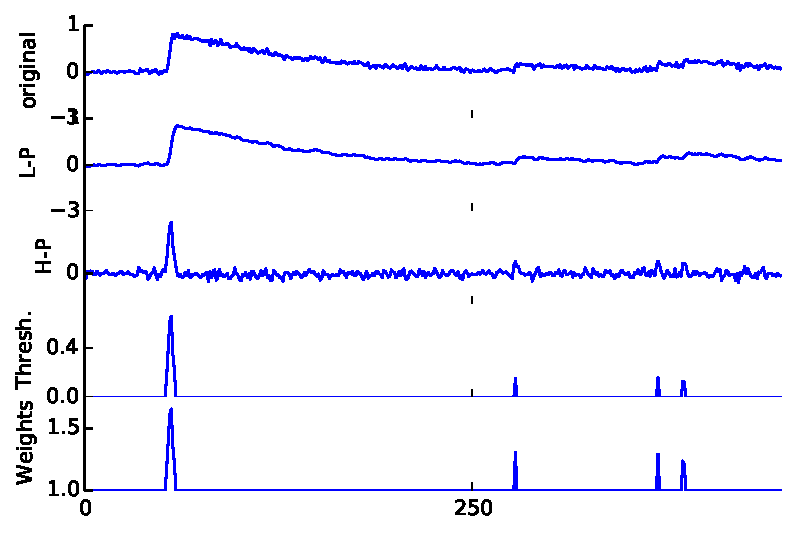
\includegraphics[width=\linewidth]{code/code/fig_filtering.png}
\end{wrapfigure} 

% Explain why we need to filter

Prior inferring the network, the fluorescent calcium time series
are smoothed using several linear and non linear filters \textcolor{red}{in order to reduce the imaging process effects. We successively apply different filters listed below.} \\



% However, the image fluorescence calcium signal is also very noisy. Thus,
% A low-pass filter (Equation \ref{eq:low-pass}) is first applied followed by a
% high-pass filter (Equation \ref{eq:high-pass}), the discrete derivative of
% the signal,
% \begin{align}
% X^\prime_{t,i} &= \sum_{l=-3}^2 c_l^k X_{t+l,i} \forall i, \label{eq:low-pass}\\
% X^{\prime\prime}_{t,i} &= X^{\prime}_{t,i} - X^{\prime}_{t-1,i} \forall i, \label{eq:high-pass}
% \end{align}
% where the $c_l^k$ coefficients were taken in one of the four
% following tuples
% $\left(c_l^1\right)_{l=-3}^2=(0, 0, 1, 1, 1, 1)$,
% $\left(c_l^2\right)_{l=-3}^2=(0, 0, 1, 1, 1, 0)$,
% $\left(c_l^3\right)_{l=-3}^2=(1, 1, 1, 1, 0, 0)$ or
% $\left(c_l^4\right)_{l=-3}^2=(0.4, 0.8, 1, 1, 0, 0)$.

\textcolor{red}{As it can be seen on \textit{fig 1}, the raw signal is very noisy and a low-pass filter is therefore applied to get a cleaner version of the signal where only true variations are kept, i.e. without noise variations. However, the choice of a low-pass filter is not unique. In the rest of the paper, we will focus on two types, the symmetrical median filter, i.e., $X_t^i \leftarrow X_{t-1}^i + X_{t}^i + X_{t+1}^i$, and an asymmetrical weighted median filter, i.e., $X_t^i \leftarrow 0.4 X_{t-3}^i + 0.6 X_{t-2}^i + 0.8 X_{t-1}^i + X_{t}^i$.}


\textcolor{red}{Considering the short delay for a communication between neurons, slow events can be neglected to retrieve direct relationships. Indeed, for a direct relationship, i.e. a neuron firing directly implying another neuron to fire, the average time is about $1ms$ or $2ms$ while the fluorescent signal time resolution is $20ms$. In order to find out which neurons are directly related, it is only necessary to look after the burst signal, or in other words, wether there is a signal variable, i.e. a burst.}

% Considering the short delay for a communication between neurons, slow events
% can be neglected to retrieve direct relationships. The average time
% delay is indeed about $1ms$ or $2ms$ while the fluorescent signal time
% resolution is $20ms$. Let us also highlight that even if two neurons are
% spatially far from each other, the delay should not exceed one time step. Thus very low frequency event can be neglected.





Connectivity information between two neurons may be retrieved from successive
and slightly delayed burst events. Direct links
between two neurons should have shorter delay between fluorescence
peaks than undirected links. However, the fluorescence signal has a slow
decay compare to its rise. Therefore, we filter those unrelevant information
with a hard thresholding filter
\begin{align}
X^{\prime\prime\prime}_{t,i} &=
{X^{\prime\prime}_{t,i}}^{0.9} \mathbb{1}(X^{\prime\prime}_{t,i} \geq \tau) \forall i
\label{eq:hard-treshold-filter}
\end{align}
where $\tau \geq 0$ is a parameter of the hard-threshold filter and the $0.9$
exponent reduce the difference between peaks values.

Then we apply on all remaining timesteps $T$ a non-linear filter based on the current
activity of the systems in order to favor the association measure when
a medium size set of neurons are firing together, while artificially
reducing the association measure in case of extreme network activity,
i.e. high when a network firing is happening and low when no neuron is
active:
\begin{equation}
X^{\prime\prime\prime\prime}_{t,i} =
\left\{
  \begin{array}{l}
    1  : r_t < 0\\
    {(X^{\prime\prime\prime}_{t,i} + 1)^{(a_t^{-1} + 1)}}^{g(r_t)} : r_t \geq 0
  \end{array}
\right.
\text{ with }
\left\{
  \begin{array}{ll}
    a_t &= \sum_{i=1}^p X^{\prime\prime\prime}_{t,i} +
                       \frac{1}{2} X^{\prime\prime\prime}_{t-1,i} \forall t \in T\\
    r_t &= \frac{a_t}{\max_{l \in T}{a_l}} \\
  \end{array}
\right.
\end{equation}
where $g(x) = b_1 I(f_4 < x < f_5) + b_2  I(f_5 \leq x < f_6) +
b_3 (I(x\leq f_4) + I(f_ 6 \leq x))$ is a piecewise continuous function of
parameters $b_1, b_2, b_3, f_4, f_5, f_6$. The coefficient were tuned
for each set $i\in\left\{1, 2, 3, 4\right\}$ of coefficient
$\left(c_l^i\right)_{l=-3}^2$.

Finally since there is a high correlation between neurons, we perform noise
filtering through a principal component analysis. From the $p$ eigen vectors,
we kept $80\%$ of the eigen vectors which have the largest eigen value. In the
context of the challenge, this assumption was deduced from ground truth of
provided networks.

\subsection{Network inference through weighted average partial correlation
            coefficients}
\label{sec:inference}

Let us denote the fluorescence calcium indicators of all neuron
as a set of random variables $X = \left\{X_1, \ldots, X_{|V|}\right\}$, which follows
a joint probability distribution $p_\mathcal{X}$, and by
$X^{-i,j}$ the set of all variables except $X_i$ and $X_j$.
Two random variables $X_i$ and $X_j$ are said to be conditionally independent
to a (possibly empty) set of random variables $Z$, denoted by $X_i \perp X_j | Z$,
if the joint conditional probability distribution factorizes
$p_{\mathcal{X}_i, \mathcal{X}_j|\mathcal{Z}} = p_{\mathcal{X}_i|\mathcal{Z}}
p_{\mathcal{X}_j|\mathcal{Z}}$.  The inference of the undirected network
can be formulated as inferring conditional dependences
$X_i \not\perp X_j | X^{-i,j}$ between all pairs $i$ and $j$ of fluorescence
signals, in other words the inferred network will be
$\hat{A}: \hat{a}_{i,j} = \mathbb{1}(X_i \not\perp X_j | X^{-i,j}), \forall i, j \in V$.

Since all neurons are assumed to be connected to at least one neuron,
we thus have by definition $X_i \not\perp X_j$. However,  two random
variables $A$ and $B$ might be dependent taken alone ($A \not\perp B$), but not
once we observe the set  $C$ of all other variables ($A \perp B | C$).
The conditioning over all other random variables $X^{-i,j}$ is thus necessary
to avoid predicting an edge when two neurons are not directly connected.

If the random variables $X$ follows a joint Gaussian distribution
$p_\mathcal{X} \sim \mathcal{N}(\mu; \Sigma)$ of mean vector $\mu$ and
covariance matrix $\Sigma$, we have the conditional independence
$X_i \perp X_j | X^{-i,j}$ if the partial correlation coefficient
\[
\rho_{X_i, X_j | X^{-i,j}}
= \frac{\Sigma^{-1}_{ij}}{\sqrt{\Sigma^{-1}_{ii} \Sigma^{-1}_{jj}}}
\]
is equal to zero (\cite{koller2009probabilistic}). The partial correlation gives
a connectivity score
$\hat{A}: \hat{a}_{i,j} = \rho_{X_i, X_j | X^{-i,j}}, \forall i, j \in V$ between all
pairs of neuron $i$ and $j$. One could retrieve an estimated graph by thresholding
the matrix $\hat{A}$.
Similarly, we also have $X_i \perp X_j$ if the Pearson correlation
coefficient
\[
\rho_{X_i,X_j} = \frac{\Sigma_{ij}}{\sqrt{\Sigma_{ii}
\Sigma_{jj}}}
\]
is equal to zero.

% Speak about why averaging
The quality of the signal filtering and network inference depends on
good hyper-parameter selection, which are themselves dependent on the properties
of the targeted network and measurement conditions, e.g. signal to noise ratio.
In order to improve robustness, a weighted average of partial correlation
matrices was estimated from the time series by varying the hard-threshold value
$\tau$ and the design of the low-pass filter (coefficients $(c_l^k)_{l=-3}^k$).



\subsection{Causal discovery methodology}
% Introduce a custom solution to make the Y matrix asymmetric
% Introduce directivity
Since partial correlation is a symmetric measure, the causal mechanism behind the
interaction ($A$ directly causes $B$, $B$ directly causes $A$ or both) can not
be directly inferred\footnote{Also note that two other causal mechanisms might be
implied while having a non-zero partial coefficient: (i) a pair of variables
is induced by a common (hidden) variable; (ii) $A$ (respectively $B$) is
conditionally correlated to a hidden variable affecting $B$ (resp. $A$)
\cite{de2004discovery}.}.

By ignoring the directivity, we systematically make a true positive and a
false positive for direct link.  Hoping to orientate
correctly the most obvious directed links, we attempt to retrieve some causal
information, i.e. the directivity of the links, by computing and stacking with
our symmetric adjacency matrix a matrix of pairwise activation heuristics.
This method computes an anti-symmetric activation score $Z$ based the
variation of fluorescence signal of a neuron $j$ due to a neuron $i$ over all
time steps:
\[
\hat{Z}: z_{ij} = \sum_{t=1}^{T - 1}
    \mathbb{1}(x_{t+1,j} - x_{t, i} \in \left[f1, f2 \right]) -
    \mathbb{1}(x_{t+1,i} - x_{t, j} \in \left[f1, f2 \right])
\]
where $f_1$ and $f_2$ are parameters of the method.

\section{Experiments}

% Datasets
To assess our method, we have used four datasets provided by the organizers
of the Connectomics challenge : \textit{normal-1, normal-2, normal-3, normal-4}.
Those datasets are time series of size $T=179500$ of image calcium from simulated
neuronal networks (\cite{stetter2012model}) with $|V|=1000$ neurons. The networks
to inferred have around 15000 edges and are similar to those
used to rank challenge participants. Note that our parameter tuning was mainly
done on the \textit{normal-1} dataset and partly on \textit{normal-4} dataset,
therefore it may justify why these networks are better retrieved despite the
fact that some might be simpler to infer.

% Metrics : ROC AUC and AUPRC
In supervised learning terms, the network inference task can be viewed as a
binary classification task where one has to correctly classify the presence
or the absence of edges of the graph. Given the ground true adjacency matrix
$A$ and a connectivity score matrix $\hat{A}$, we assess the accuracy of the
network inference method using the area under the ROC curve (ROC AUC)
and the area under the precision-recall curve (AUPRC)
(\cite{schrynemackers2013protocols}). Since neurons are not self-connected
($(i, i) \not \in E, \forall i \in V$) and some inference methods could
give maximal scores to the diagonal of $\hat{A}$, e.g. Pearson
correlation, we set those elements to the minimum of $\hat{A}$ prior
assessment.


% TODO
%   - discussions about the results
%   - discussions about the metrics (Gilles' text)

For the directory method, only filters defined by Equations
\ref{eq:low-pass}, \ref{eq:high-pass} and \ref{eq:hard-treshold-filter} were
used.

\begin{table}[htb]
\centering
\caption{Inverse correlation (ROC). Improvement of each stage of our approach. Note that we choose the
         \textit{best} threshold (\textcolor{red}{for now 0.11}) for stages 1 to 4.}
\begin{tabular}{*{5}{l}}
\toprule
Stage               & normal-1 & normal-2 & normal-3 & normal-4 \\
\midrule
Nothing             & 0.777 & 0.767 & 0.772 & 0.774 \\
PCA                 & 0.780 & 0.770 & 0.776 & 0.777 \\
Weights             & 0.780 & 0.769 & 0.776 & 0.777 \\
Weights + PCA       & 0.783 & 0.772 & 0.779 & 0.780 \\
H-T                 & 0.893 & 0.891 & 0.891 & 0.886 \\
H-T + PCA           & 0.894 & 0.892 & 0.891 & 0.886 \\
H-T + Weights       & 0.899 & 0.897 & 0.896 & 0.891 \\
H-T + Weights + PCA & 0.900 & 0.898 & 0.896 & 0.892 \\
P-P                 & 0.925 & 0.925 & 0.924 & 0.923 \\
P-P + PCA           & 0.926 & 0.926 & 0.925 & 0.923 \\
P-P + Weights       & 0.931 & 0.930 & 0.928 & 0.927 \\
P-P + Weights + PCA & 0.932 & 0.931 & 0.930 & 0.928 \\
Averaging (PCA)     & 0.943 & 0.942 & 0.942 & 0.939 \\
Stacking            & 0.944 & 0.943 & 0.942 & 0.940 \\
\bottomrule
\end{tabular}
\end{table}


\begin{table}[htb]
\centering
\caption{Inverse correlation (P-R). Improvement of each stage of our approach. Note that we choose the
         \textit{best} threshold (\textcolor{red}{for now 0.11}) for stages 1 to 4.}
\begin{tabular}{*{5}{l}}
\toprule
Stage               & normal-1 & normal-2 & normal-3 & normal-4 \\
\midrule
Nothing             & 0.070 & 0.064 & 0.068 & 0.072\\
PCA                 & 0.076 & 0.070 & 0.075 & 0.079\\
Weights             & 0.074 & 0.067 & 0.072 & 0.076\\
Weights + PCA       & 0.080 & 0.073 & 0.079 & 0.083\\
H-T                 & 0.264 & 0.260 & 0.269 & 0.241\\
H-T + PCA           & 0.266 & 0.263 & 0.273 & 0.244\\
H-T + Weights       & 0.280 & 0.273 & 0.281 & 0.251\\
H-T + Weights + PCA & 0.284 & 0.278 & 0.285 & 0.255\\
P-P                 & 0.322 & 0.324 & 0.323 & 0.312\\
P-P + PCA           & 0.347 & 0.352 & 0.355 & 0.341\\
P-P + Weights       & 0.333 & 0.334 & 0.327 & 0.313\\
P-P + Weights + PCA & 0.364 & 0.366 & 0.359 & 0.344\\
Averaging           & 0.403 & 0.404 & 0.398 & 0.388\\
Stacking            & 0.404 & 0.405 & 0.399 & 0.389\\
\bottomrule
\end{tabular}
\end{table}


\begin{table}[H]
\centering
\caption{Comparison (ROC) with other methods (for now, $t = 0.11$)}
\begin{tabular}{*{5}{l}}
\toprule
Methods             & normal-1 & normal-2 & normal-3 & normal-4 \\
\midrule
Correlation (best)         & 0.886 & 0.884 & 0.891 & 0.877\\
Partial correlation (best) & 0.932 & 0.931 & 0.930 & 0.928 \\
Our approach               & 0.943 & 0.942 & 0.942 & 0.939 \\
GENIE3                     & & & & \\
GTE                        & 0.890 & 0.893 & 0.894 & 0.873 \\
Directivity                & 0.535 & 0.526 & 0.533 & 0.535 \\
Our approach + dir         & 0.944 & 0.943 & 0.942 & 0.940\\
\bottomrule
\end{tabular}
\end{table}

\begin{table}[htb]
\centering
\caption{Comparison (P-R) with other methods (for now, $t = 0.11$)}
\begin{tabular}{*{5}{l}}
\toprule
Methods             & normal-1 & normal-2 & normal-3 & normal-4 \\
\midrule
Correlation (best)         & 0.153 & 0.145 & 0.170 & 0.132 \\
Partial correlation (best) & 0.364 & 0.366 & 0.359 & 0.344 \\
Our approach (best)        & 0.403 & 0.404 & 0.398 & 0.388 \\
GENIE3                     & & & & \\
GTE                        & 0.171 & 0.174 & 0.197 & 0.142 \\
Directivity                & 0.012 & 0.012 & 0.012 & 0.012 \\
Our approach + dir         & 0.404 & 0.405 & 0.399 & 0.389 \\
\bottomrule
\end{tabular}
\end{table}



\section{Conclusion}

In previous study \cite{shipley2002cause}, it has been suggested to
consider correlation coefficients of all possible orders,
i.e. conditioned on every subsets of the set of $p-2$ other variables. This
would take into account multiple indirect paths between a given pair of
variables.

% Possible extensions
% partial autocorrelation function (sometimes "partial correlation function")
% conditional independence test
% Speak about the complexity and parallelization of the methods




\begin{scriptsize}

\paragraph{Acknowledgements.} A. Joly and G. Louppe are research fellows of
the FNRS, Belgium.  A. Sutera is  is recipient of
a F.R.I.A. fellowship of F.R.S.-FNRS, Belgium.
This work is supported by PASCAL2 and the IUAP DYSCO, initiated by the
Belgian State, Science Policy Office.

\end{scriptsize}

\newpage
\clearpage

% We allow the bibliography to be added on top of the 6 pages.
% Supplementary material may be added in the form or a URL pointed to from
% the paper.
\bibliography{references}

\newpage
\clearpage

\appendix

\section{Supplementary results}

\begin{table}[htbp]
\centering
\caption{Correlation (ROC). Improvement of each stage of our approach. Note that we choose the
         \textit{best} threshold (\textcolor{red}{for now 0.11}) for stages 1 to 4.}
\begin{tabular}{*{5}{l}}
\toprule
Stage               & normal-1 & normal-2 & normal-3 & normal-4 \\
\midrule
Nothing             & 0.681 & 0.699 & 0.683 & 0.681\\
Weights             & 0.695 & 0.713 & 0.697 & 0.694\\
H-T                 & 0.876 & 0.873 & 0.877 & 0.869\\
H-T + Weights       & 0.886 & 0.884 & 0.891 & 0.877\\
P-P                 & 0.857 & 0.850 & 0.843 & 0.832\\
P-P + Weights       & 0.826 & 0.823 & 0.817 & 0.799\\
\bottomrule
\end{tabular}
\end{table}

\begin{table}[htbp]
\centering
\caption{Correlation (P-R). Improvement of each stage of our approach. Note that we choose the
         \textit{best} threshold (\textcolor{red}{for now 0.11}) for stages 1 to 4.}
\begin{tabular}{*{5}{l}}
\toprule
Stage               & normal-1 & normal-2 & normal-3 & normal-4 \\
\midrule
Nothing             & 0.028 & 0.028 & 0.025 & 0.026\\
Weights             & 0.031 & 0.030 & 0.027 & 0.028\\
H-T                 & 0.143 & 0.128 & 0.150 & 0.129\\
H-T + Weights       & 0.153 & 0.145 & 0.170 & 0.132\\
P-P                 & 0.100 & 0.087 & 0.079 & 0.083\\
P-P + Weights       & 0.079 & 0.071 & 0.067 & 0.064\\
\bottomrule
\end{tabular}
\end{table}

\end{document}
